
\section{Architecture}
\label{sec:Architecture}
To maximize performance within a constrained resources, Ling 2.0 series uniformly adopts a MoE architecture~\citep{shazeer2017outrageously,deepseekai2024deepseekv3technicalreport}. It integrates aux-loss-free load balancing strategy~\citep{deepseekai2024deepseekv3technicalreport} and Multi-Token Prediction (MTP)~\citep{gloeckle2024better,deepseekai2024deepseekv3technicalreport} to optimize the training process. Furthermore, our architectural decisions are grounded in systematic scaling law experiments~\citep{tian2025greaterleveragescalinglaws} that verify the reliable extrapolation of key architectural details, thus enabling efficient architecture iteration and principled design choices. 

\subsection{Basic Architecture}
\label{sec:basic_arch}
The Ling 2.0 series comprises three MoE models of varying scales: \texttt{Ling-mini-2.0}, \texttt{Ling-flash-2.0}, and \texttt{Ling-1T}, covering total parameter counts from 16B up to 1T. Key architectural details of the models are summarized in Table~\ref{tab:model-specs}.

Ling 2.0 models adopt a unified ``high-sparsity, fine-grained'' design: each model is configured with 256 routed experts, activates 8 experts plus 1 shared expert, yielding an overall activation ratio of approximately 3.5\%. Our scaling laws analysis~\citep{tian2025greaterleveragescalinglaws} indicates that continuously increasing sparsity yields significant performance gains~\citep{kimiK2}. Concurrently, the fine-grained setting of activating 8 experts presents a superior balance between training speed and model performance, while the inclusion of one shared expert was identified as an optimal design heuristic through our extensive experiments. Additionally, we designate the initial 1, 1, and 4 layers of the three models, respectively, as dense layers. This approach reduces the total parameter count while maintaining equivalent model performance and improving routing balance. 

In the attention layers, Ling 2.0 models employ standard grouped-query attention (GQA)~\citep{ainslie2023gqa} with 8, 16, or 32 key-value heads to reduce KV cache size during decoding; it employs SwiGLU and RMSNorm with pre-normalization to improve representational efficiency and stability. We further introduce QKNorm~\citep{henry2020query} to enhance training robustness, which we verify to significantly improve stability under low-precision training. Furthermore, we implement Partial RoPE~\citep{su2024roformer}, applying rotary position embeddings only to the first 64 dimensions of the attention heads, to bolster the model's length extrapolation capabilities. 

Ling 2.0 extends the Ling 1.5 vocabulary and uses byte-level byte-pair encoding, BBPE~\citep{shibata1999byte, sennrich2015neural}, with a 156K token vocabulary to enhance multilingual performance.


\begin{table}[h!]
\centering
\caption{\textbf{Key architectural configurations and training hyperparameters of the Ling 2.0 series.}} %
\vspace{-0.1cm}
\label{tab:model-specs} %
\small
\begin{tabular}{l *{3}{>{\centering\arraybackslash}p{2.5cm}}}
\toprule
                        & \textbf{\texttt{\texttt{Ling-mini-2.0}}} & \textbf{\texttt{Ling-flash-2.0}} & \textbf{\texttt{Ling-1T}} \\
\midrule
\# Layers                  & 20                & 32                 & 80              \\
\# Experts (total)         & 256               & 256                & 256             \\
\# Experts Active per Token& 8                 & 8                  & 8               \\
\# Shared Experts          & 1                 & 1                  & 1               \\
\# Attention Heads         & 16                & 32                 & 64              \\
\# Dense Layers  & 1                 & 1                  & 4               \\
Hidden Size                & 2{,}048   & 4{,}096   & 8{,}192   \\
Intermediate Size          & 5{,}120   & 9{,}216   & 18{,}432  \\
Expert Intermediate Size  & 512       & 1{,}024   & 2{,}048    \\
Total Parameters (B)       & 16              & 103              & 1000            \\
Activated Parameters (B)    & 1.4               & 6.1                & 51.0            \\
\midrule
Learning Rate       & $3.36\times10^{-4}$              & $2.61\times10^{-4}$              & $1.86\times10^{-4}$            \\
Batch Size      & $4{,}400$               & $8{,}352$                & $18{,}144$           \\
\bottomrule
\end{tabular}
\end{table}

\subsection{Model Optimization}
To further improve the training efficiency and final performance of Ling 2.0, we incorporate the aux-loss-free load balancing strategy and Multi-Token Prediction (MTP).

\paratitle{Load Balancing Strategy. }
\label{sec:load_balance}
Based on systematic experiments, Ling 2.0's routing balance strategy follows a design similar to DeepSeek-V3~\citep{deepseekai2024deepseekv3technicalreport}. We choose an aux-loss-free balance strategy to jointly encourage expert specialization and load balancing, and we apply router gate scaling to improve training stability. The scaling factor is set to 2.5 to stabilize the root mean square of the gate outputs. We slightly modify the bias update strategy, keeping the bias centered around zero~\citep{liu2025muon}. Concretely, the aux-free bias is updated as:
$b_i = b_i + u \times \bigl(\operatorname{sign}(e_i) - \operatorname{mean}(\operatorname{sign}(e))\bigr),$
where $u$ is the update rate, $b_i$ is the bias of the $i$-th expert, and $e_i$ is that expert's violation error.
In addition, we adopt a dropless routing strategy to ensure model performance, alongside group routing to improve training efficiency without any performance degradation.


\paratitle{Multi Token Prediction. }
\label{sec:mtp}
To enhance model performance and inference efficiency, Ling 2.0 natively integrates MTP~\citep{gloeckle2024better,deepseekai2024deepseekv3technicalreport}  as an auxiliary training objective. Through rigorous validation of its effectiveness and extrapolability, we found that MTP consistently improves performance on code and math tasks across different model scales. Considering the scaling trends of MTP hyperparameters and training efficiency across various model sizes, we introduce one MTP layer for each model scale and set the MTP loss weight to 0.1. 
To address the additional computational overhead introduced by MTP, we performed a detailed performance analysis and implemented fine-grained Pipeline Parallelism (PP) partitioning for the MTP module within the Megatron training framework. This optimization significantly mitigates the performance overhead from MTP, ensuring high training throughput (see Section~\ref{sec:infra} for details).

\subsection{Ling Scaling Laws}
\label{sec:scaling_law}

Ling 2.0 series was conceived from the outset with the long-term goal of training trillion-parameter foundation models. 
To this end, we establish the Ling Scaling Laws~\citep{tian2025greaterleveragescalinglaws} to guide hyperparameter and architecture choices. 
The framework also provides the foundation for a standardized experimental pipeline, ensuring reliable extrapolation of findings to computational scales over 100x larger.
Specifically, the Ling Scaling Laws serve two critical functions:
\begin{itemize}
\item 
\textbf{Principled Design for Trillion-Parameter Models:} 
The laws determine the hyperparameters and architectural settings for Ling 2.0, ensuring near-optimal architectural efficiency.
\item \textbf{Efficient Innovation at Minimal Cost:}
A standardized pipeline are provided to validate novel ideas and emerging technologies for Ling 2.0 at just 1\% of the full training compute cost. 
\end{itemize}

\subsubsection{Scaling Laws for Optimal Hyper-parameters}
\label{sec:scaling4parametres}
To ensure that the Ling 2.0 series can be trained stably under appropriate hyperparameters, we first derived scaling laws for optimal MoE hyperparameters. Previous studies~\citep{bi2024deepseek, team2025every} has shown that the optimal learning rate ($\eta$) and batch size ($B$) are primarily determined by the total compute budget ($C$). Accordingly, we conducted hyperparameter searches over nearly a thousand experiments across compute scales up to $3e{20}$ FLOPs, using a Warmup–Stable–Decay (WSD) scheduler~\citep{hu2024minicpm}.  
To simplify analysis, we initially fixed the MoE architecture to 64 experts (4 active) plus 1 shared expert. After removing outliers, we selected optimal and near-optimal\footnote{``near-optimal'' is defined as configurations whose loss is within 0.25\% of the minimum at a given compute budget.} configurations for fitting. From these data, we fit power-law relationships between compute $C$ and the optimal batch size $B_{\mathrm{opt}}$ and learning rate $\eta_{\mathrm{opt}}$, and verified that the resulting laws remain near-optimal under different activation ratios. The fitting process and fitted parameters is shown in Figure~\ref{fig:hyper-and-modeldata-scaling-a}.

Our analysis reveals a key difference between MoE and dense models in hyperparameter selection: at larger compute scales, MoEs tend to use larger batch sizes and relatively lower learning rate. We attribute this phenomenon to MoEs' sparse gradient updates: since only a subset of tokens in each batch contributes to the gradient update for any given expert, a larger batch size is necessary to ensure stable and effective training. These validated scaling laws provided a reliable foundation, enabling the efficient training of the Ling 2.0 models with near-optimal hyperparameters. 

\begin{figure}[t!]
    \centering
    \begin{subfigure}[b]{0.5\textwidth}
        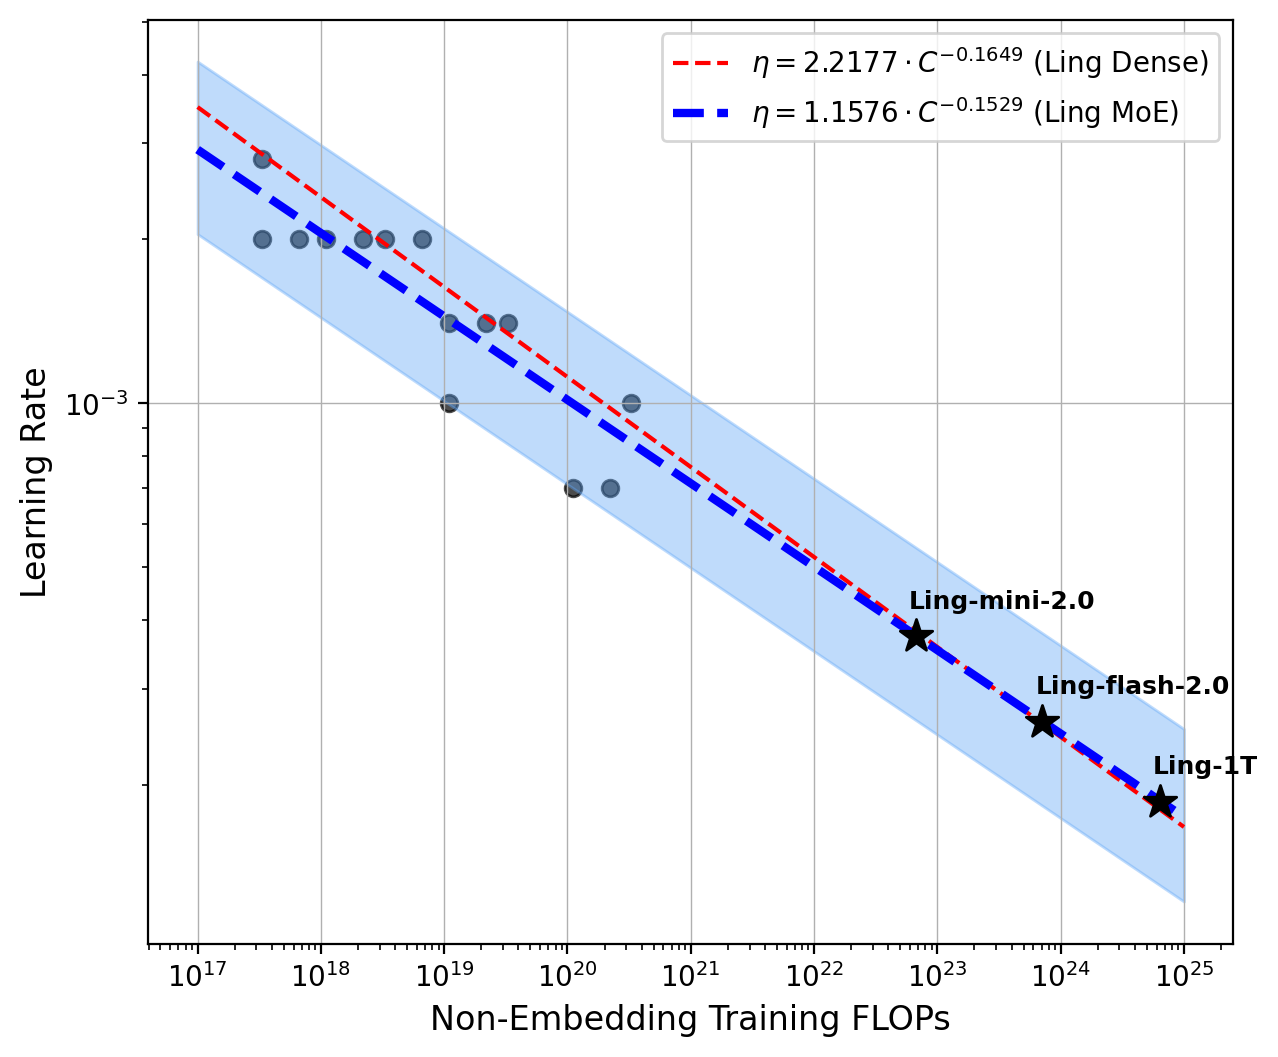
\includegraphics[width=0.49\textwidth]{figs/lr-train_loss_smooth_4096-1.001-0.34-wLing.png}
        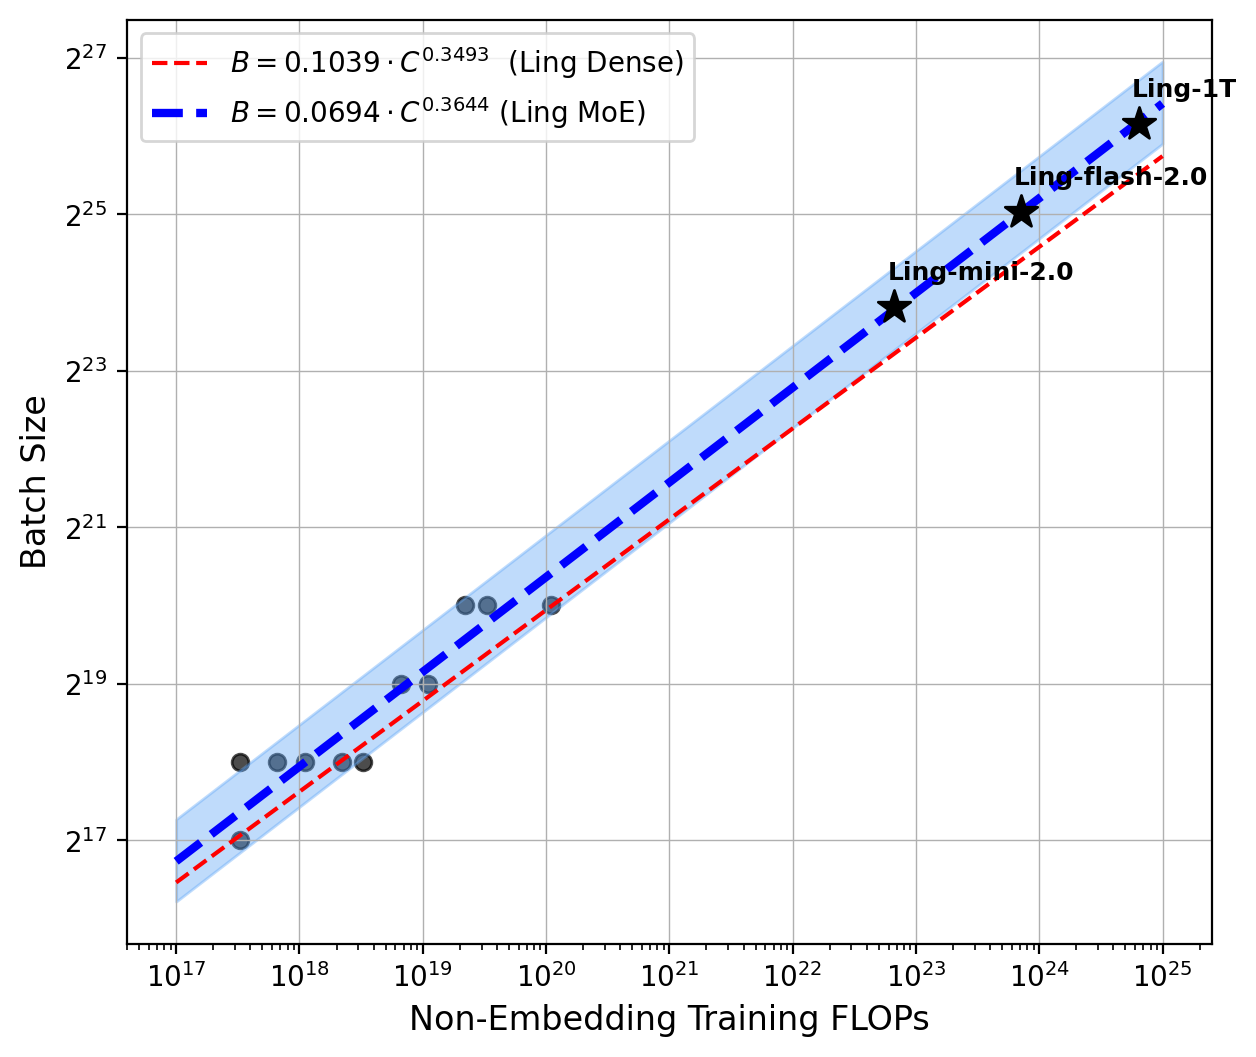
\includegraphics[width=0.48\textwidth]{figs/bs-train_loss_smooth_4096-1.001-0.34-wLing.png}
        \caption{Scaling laws for optimal hyperparameters}
        \label{fig:hyper-and-modeldata-scaling-a}
    \end{subfigure}
    \hfill 
    \begin{subfigure}[b]{0.49\textwidth} 
        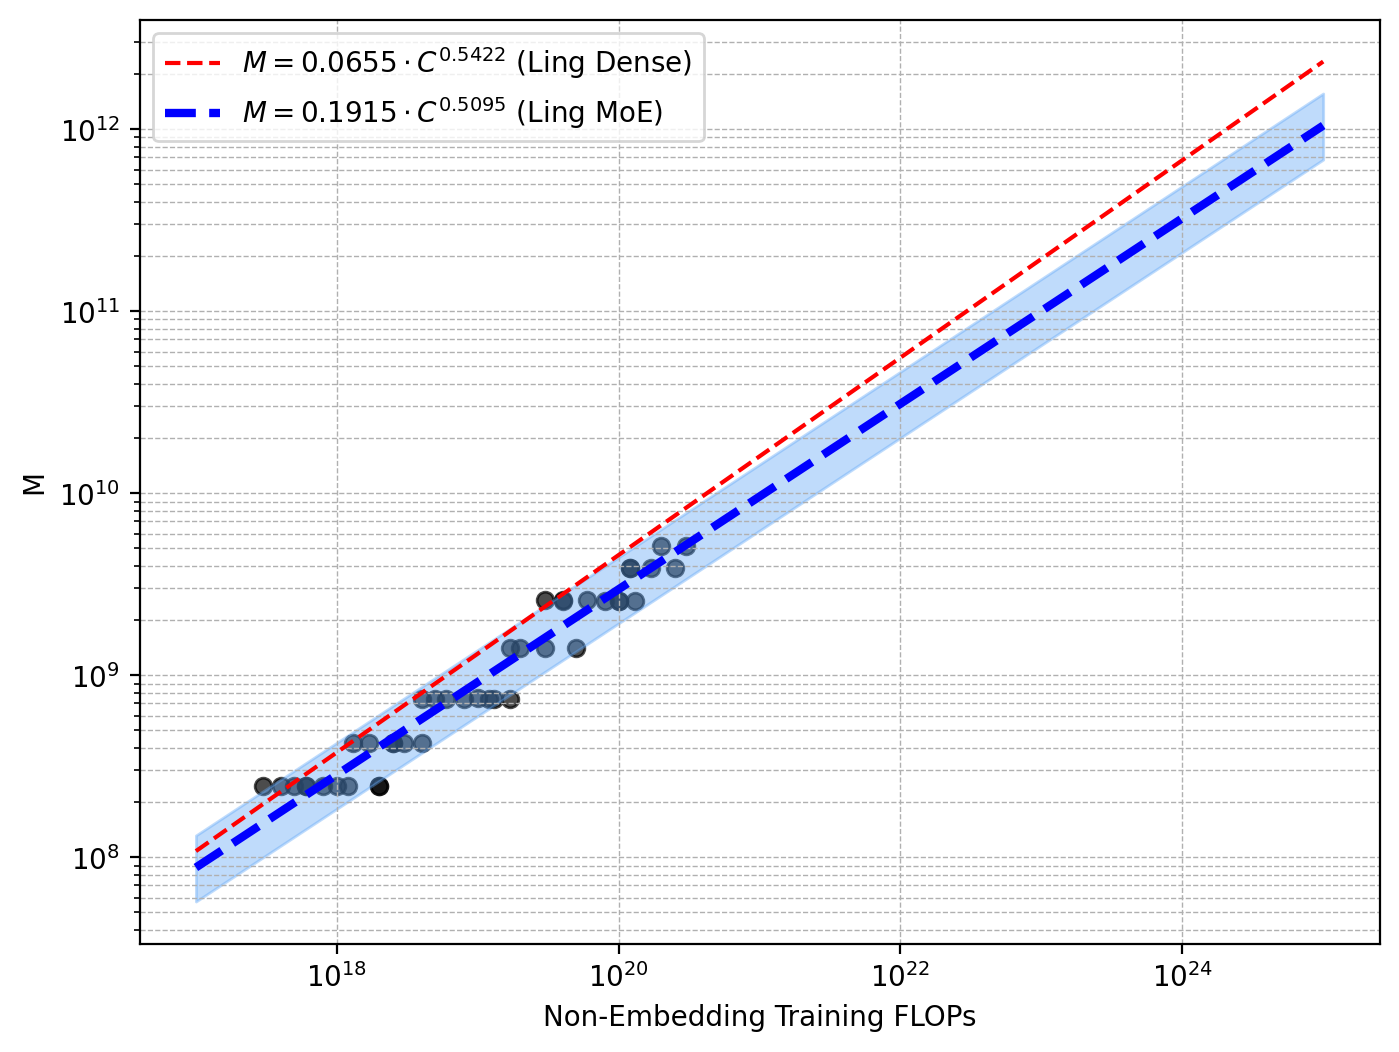
\includegraphics[width=0.49\textwidth,height=0.415\textwidth]{figs/M-train_loss_smooth_unfix_1-1.0025-2.png}
        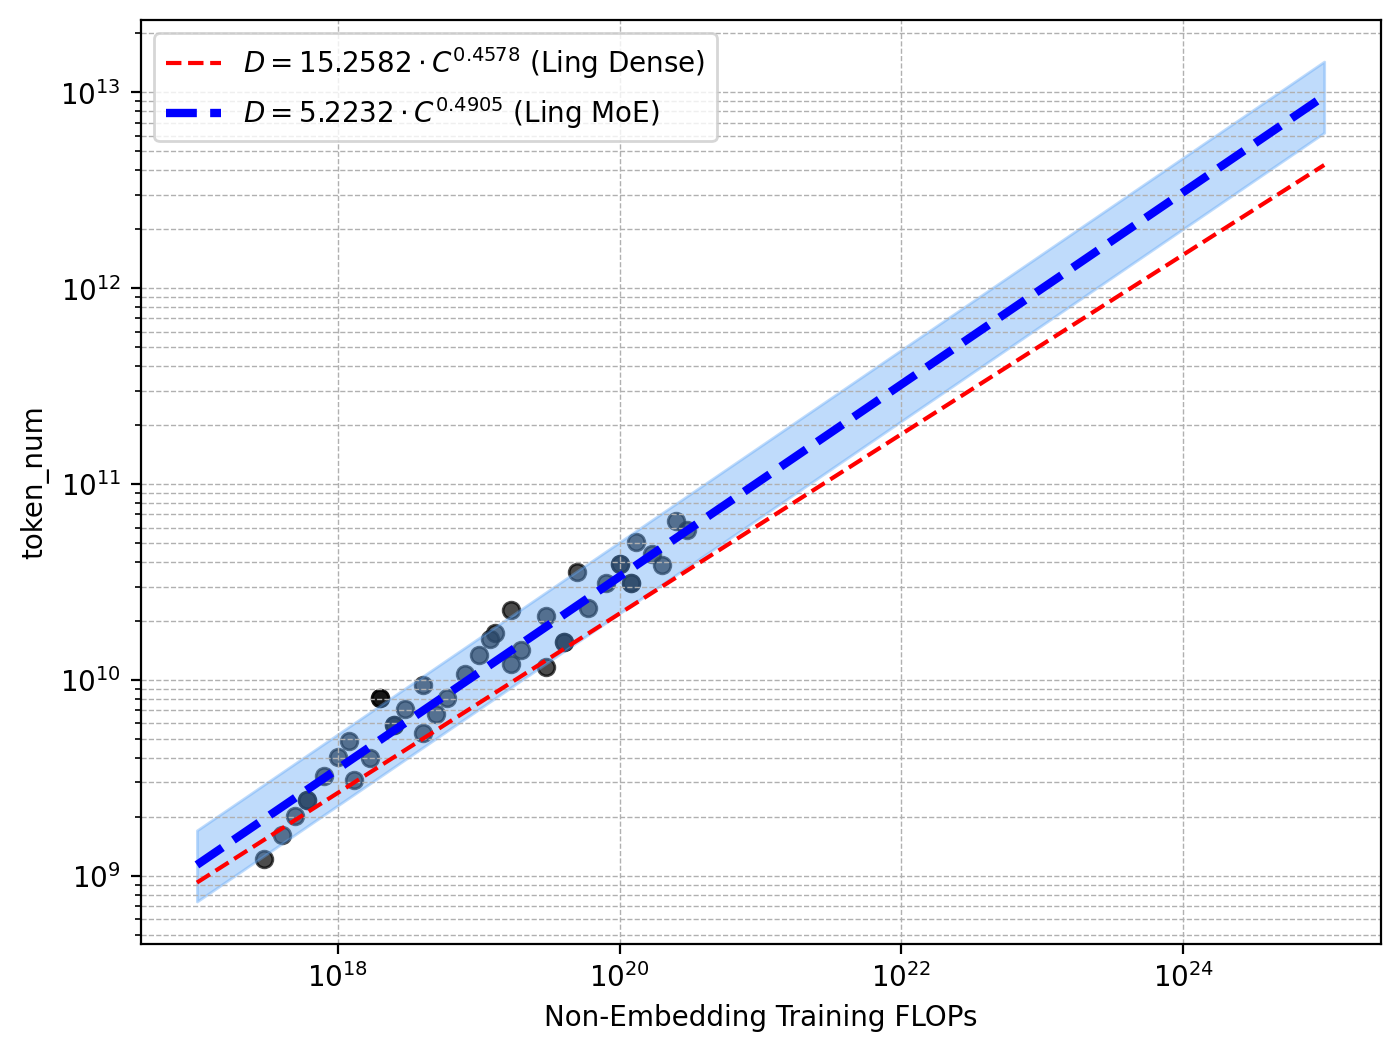
\includegraphics[width=0.49\textwidth,height=0.415\textwidth]{figs/token_num-train_loss_smooth_unfix_1-1.0025-2.png}
        \caption{Scaling laws for optimal model-data allocation}
        \label{fig:hyper-and-modeldata-scaling-b}
    \end{subfigure}
    \caption{{Scaling laws for optimal hyperparameters and optimal model-data allocation.} Blue and red lines represent the fitted laws for MoE and dense models, respectively, derived on the same training dataset. Gray circles are the experimental data points used for fitting.}
    \label{fig:hyper-and-modeldata-scaling}
\end{figure}

Furthermore, to gain deeper insight into the differing training dynamics of MoE and dense models, we analyzed the optimal allocation for training data ($D$) and model parameters ($M$, i.e., FLOPs per token) under different compute budgets ($C = M\cdot D$). As shown in Figure~\ref{fig:hyper-and-modeldata-scaling-b}, our findings indicate that for any given compute budget, the optimal MoE model has fewer parameters ($M_{\text{opt}}$) but is trained on more data ($D_{\text{opt}}$) compared to its optimal dense counterpart. This conclusion suggests that MoE architectures possess a larger effective capacity, enabling them to efficiently process more training data with fewer parameters, which offers a significant efficiency advantage in real-world scenarios where data is abundant but computational resources are limited. 



\subsubsection{Scaling Laws for MoE Architectural Efficiency}
\label{sec:scaling4moe}
To guide the architectural design of the Ling 2.0, we systematically derived scaling laws for MoE architectural efficiency. We introduce \textit{efficiency leverage} (EL) as our primary metric, defined as the ratio of computational cost required for a dense model to that of an MoE model to reach an equivalent performance level (e.g., identical validation loss). Our investigation systematically analyzes the influence of key architectural dimensions on EL, including the expert activation ratio, expert granularity, the proportion of shared experts, and others. We then integrate the empirical findings into a unified scaling law that predicts EL as a function of the MoE configuration, offering a practical framework for designing efficient MoEs. This large-scale empirical study, based on \textit{over 300 models with up to 28B parameters}, reveals several core principles governing MoE efficiency:

\begin{enumerate}
\item \textbf{Activation ratio is the primary driver of efficiency.}
EL is predominantly determined by the expert activation ratio, following a robust power law: efficiency gains increase as sparsity increases (i.e., as the activation ratio decreases). Illustrated in Figure~\ref{fig:IsoFlops-scaling} (left), this relationship remains consistent and quantifiable even at extremely low activation ratios, such as 1/128.

\item \textbf{Expert granularity acts as a nonlinear modulator.}
Beyond the dominant activation effect, expert granularity induces a log-polynomial adjustment to EL that is largely independent of the total compute budget, implying a stable optimal range for the number of activated experts. Our experiments identify this optimal range as 8--12, as shown in Figure~\ref{fig:IsoFlops-scaling} (right).

\item \textbf{Compute budget has an amplification effect.}
Crucially, EL for a given MoE architecture is not fixed; it scales with the training compute budget following another power law. This highlights the substantial potential of MoE in large-scale pretraining: as compute investment increases, the efficiency advantage becomes increasingly pronounced. 

\item \textbf{Other architectural factors have secondary effects.}
Factors such as the arrangement of shared expert or MoE layers have relatively minor effects. These factors typically admit broadly applicable, near-optimal settings and do not require fine-grained tuning across scenarios.

\end{enumerate}


\begin{figure}[t!]
    \centering
    \begin{subfigure}[b]{0.59\textwidth}
        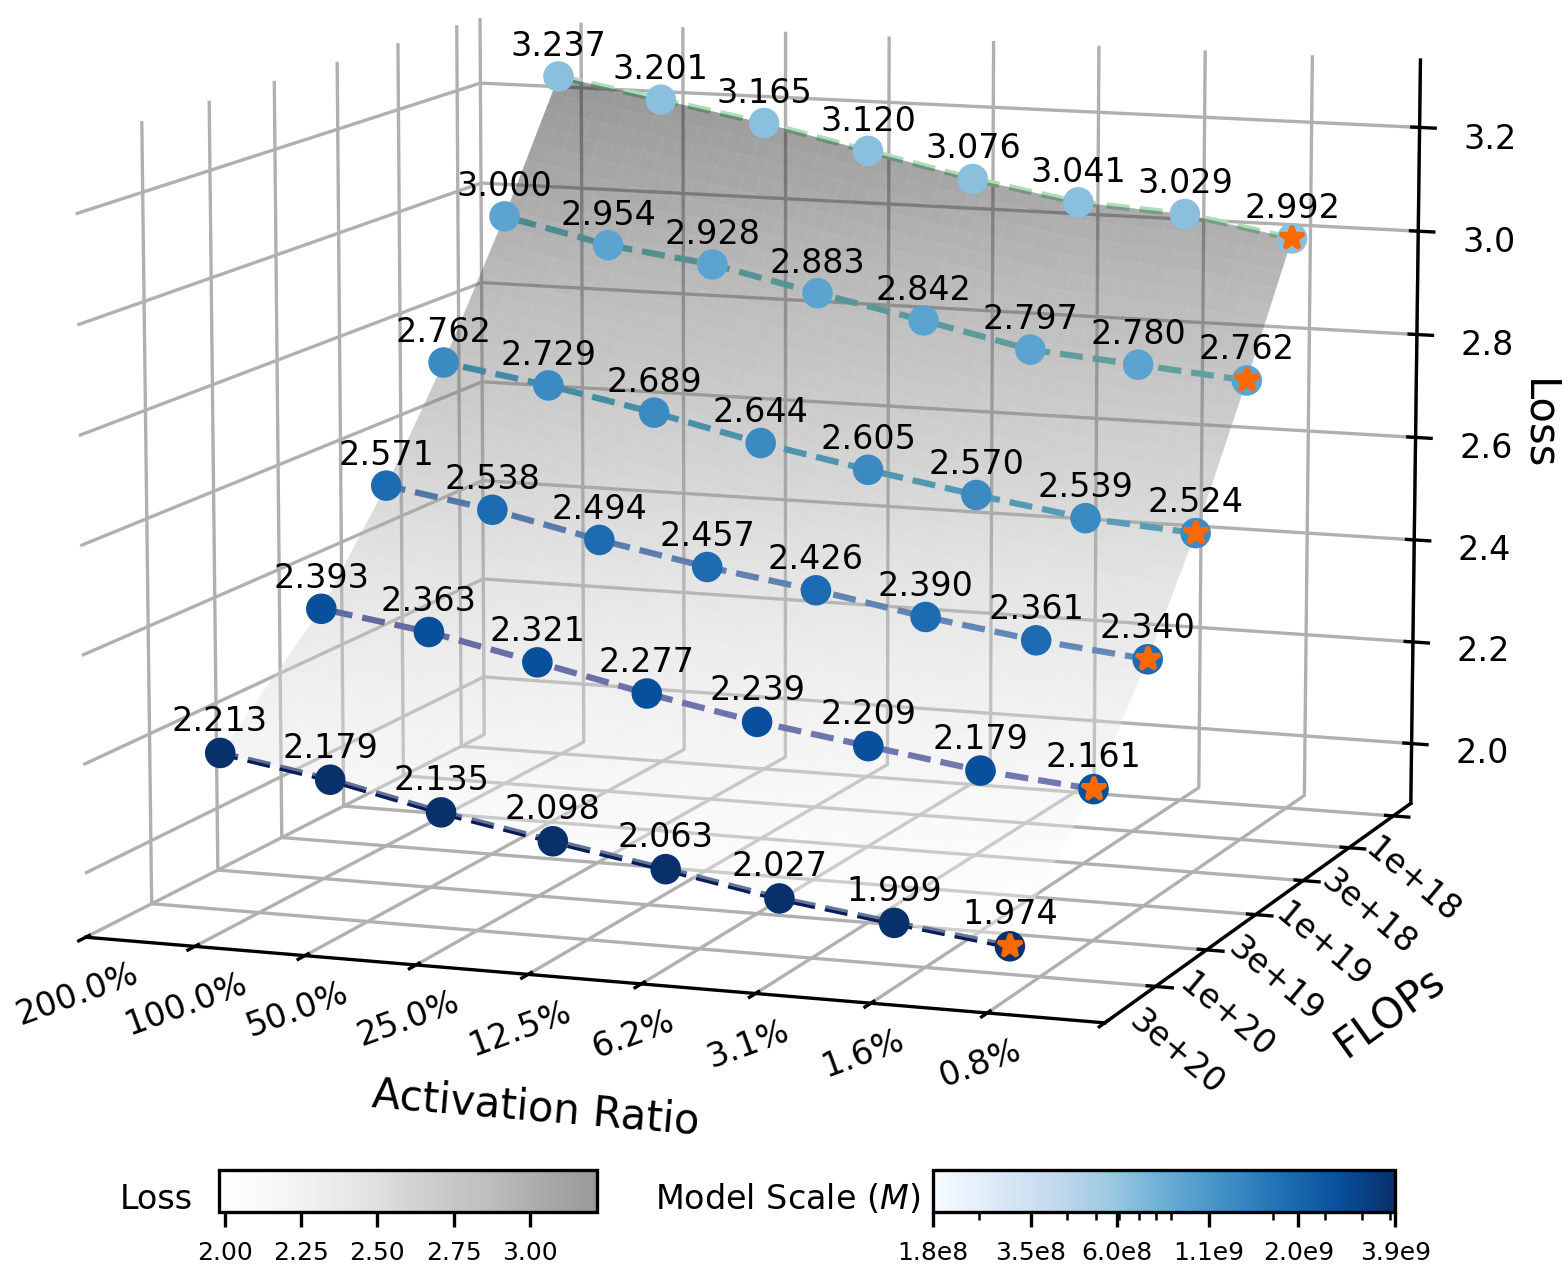
\includegraphics[width=0.5\textwidth]{figs/scaling_act_ratio.png}
        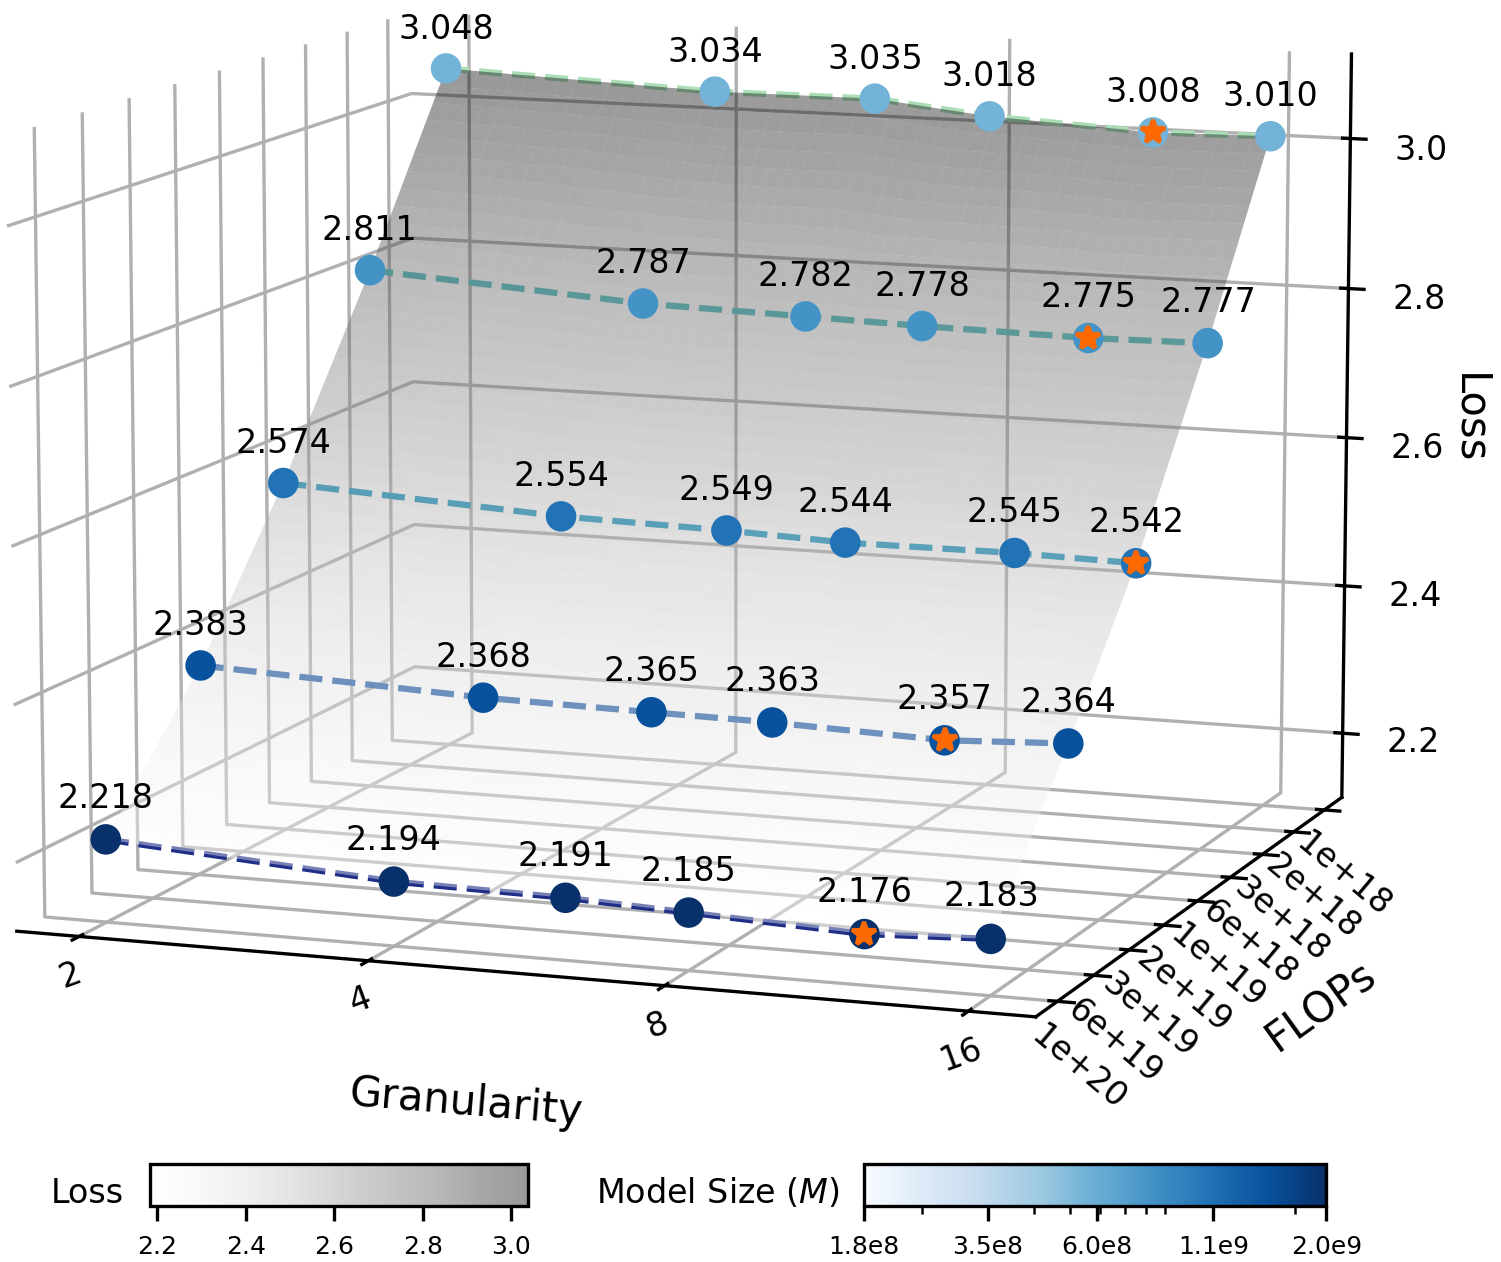
\includegraphics[width=0.47\textwidth]{figs/scaling_moe_router_topk.png}
        \caption{IsoFLOPs curves for varying activation ratio and expert granularity.}
        \label{fig:IsoFlops-scaling}
    \end{subfigure}
    \hfill 
    \begin{subfigure}[b]{0.4\textwidth} 
        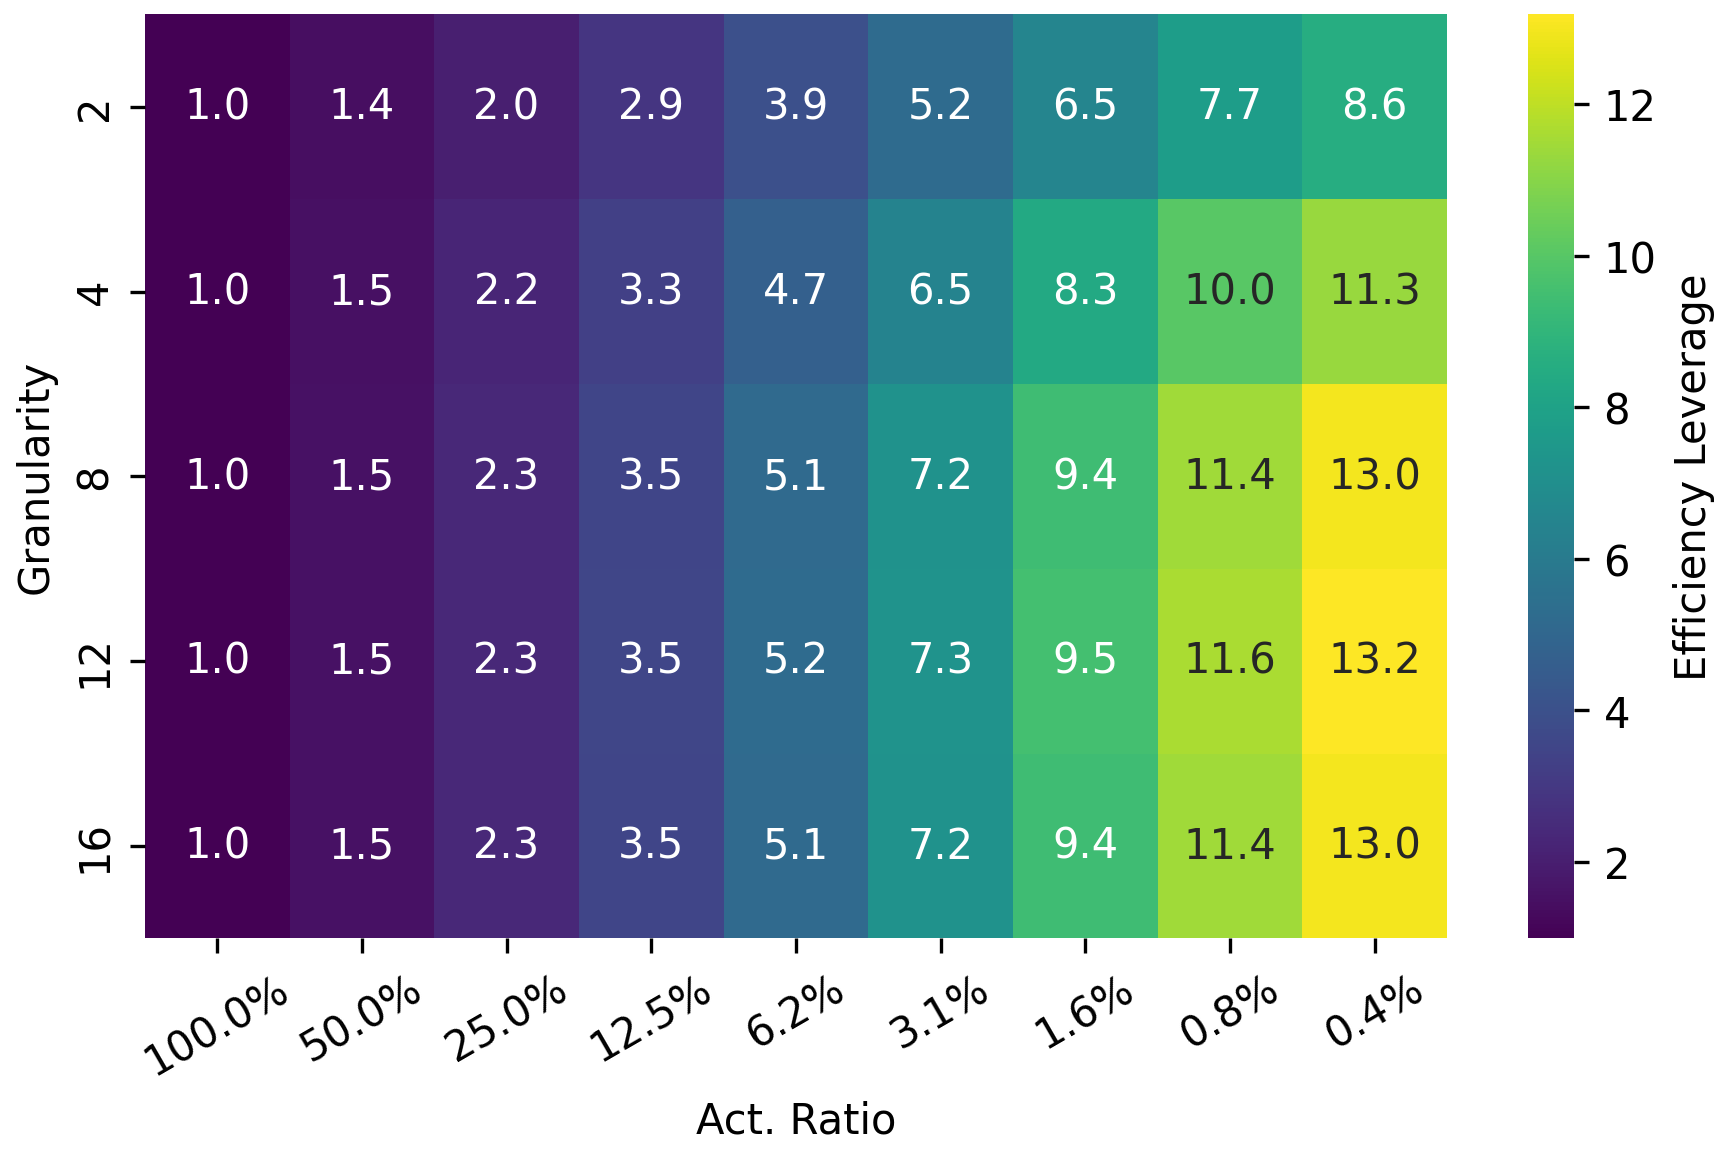
\includegraphics[width=0.9\textwidth,height=0.58\textwidth]{figs/lever_hotmap_1e+22.png}
        \caption{Estimated efficiency leverage (EL)}
        \label{fig:lever-1e22}
    \end{subfigure}
    \caption{{Impact of the MoE architectural configuration on loss and efficiency leverage (EL).}}
    \label{fig:scaling}
\end{figure}


Combining these insights, we derive a unified EL scaling law that integrates the effects of the compute budget ($C$), activation ratio ($A$), and expert granularity ($G$):
\begin{equation}
\begin{aligned}
    {EL}(A,G,C) &= \hat A^{\alpha + \gamma(\log G)^2 + \beta \log G}, \\
\end{aligned}
\label{eq:all}
\end{equation}
where $\hat{A}$ is a saturating transformation of the activation ratio $A$, as defined in \cite{clark2022unified}.
The exponent $\alpha = a + d \cdot \log C$ models the compute-dependent scaling. Here, $d > 0$ quantifies the amplification of EL at larger compute scales, while $a$ represents the baseline scaling exponent. The parameters $\beta$ and $\gamma$ define the log-polynomial modulation from expert granularity $G$, capturing the observed optimal range.
We fit Eq.~\ref{eq:all} using Huber loss and BFGS optimization~\citep{hoffmann2022training}, and experimentally validated the scaling on \texttt{\texttt{Ling-mini-2.0}}. As an example, Figure~\ref{fig:lever-1e22} presents the predicted EL landscape at $1e{22}$ FLOPs, highlighting the optimal architectural region. Based on these results, all Ling 2.0 models adopt a high-sparsity, fine-granularity design: 256 routing experts with 8 activated per token plus one shared expert, yielding a 3.5\% overall activation ratio. 
The Ling scaling law predicts \textbf{{over 7× efficiency leverage}} for this architectural configuration, which we empirically confirm on the Ling 2.0 series.





\subsubsection{{Ling Wind Tunnel Experiments for Efficient Innovation}}
The Ling Scaling Laws not only dictate the specific training and architectural parameters but, more importantly, guide the experimental and iterative paradigm of the Ling project with longtermism. To facilitate efficient innovation at minimal cost, we design the ``Ling Wind Tunnel Experiments'' system based on these scaling laws.

\begin{figure}[t!]
    \centering
    \begin{subfigure}[b]{0.55\textwidth}
        \centering
        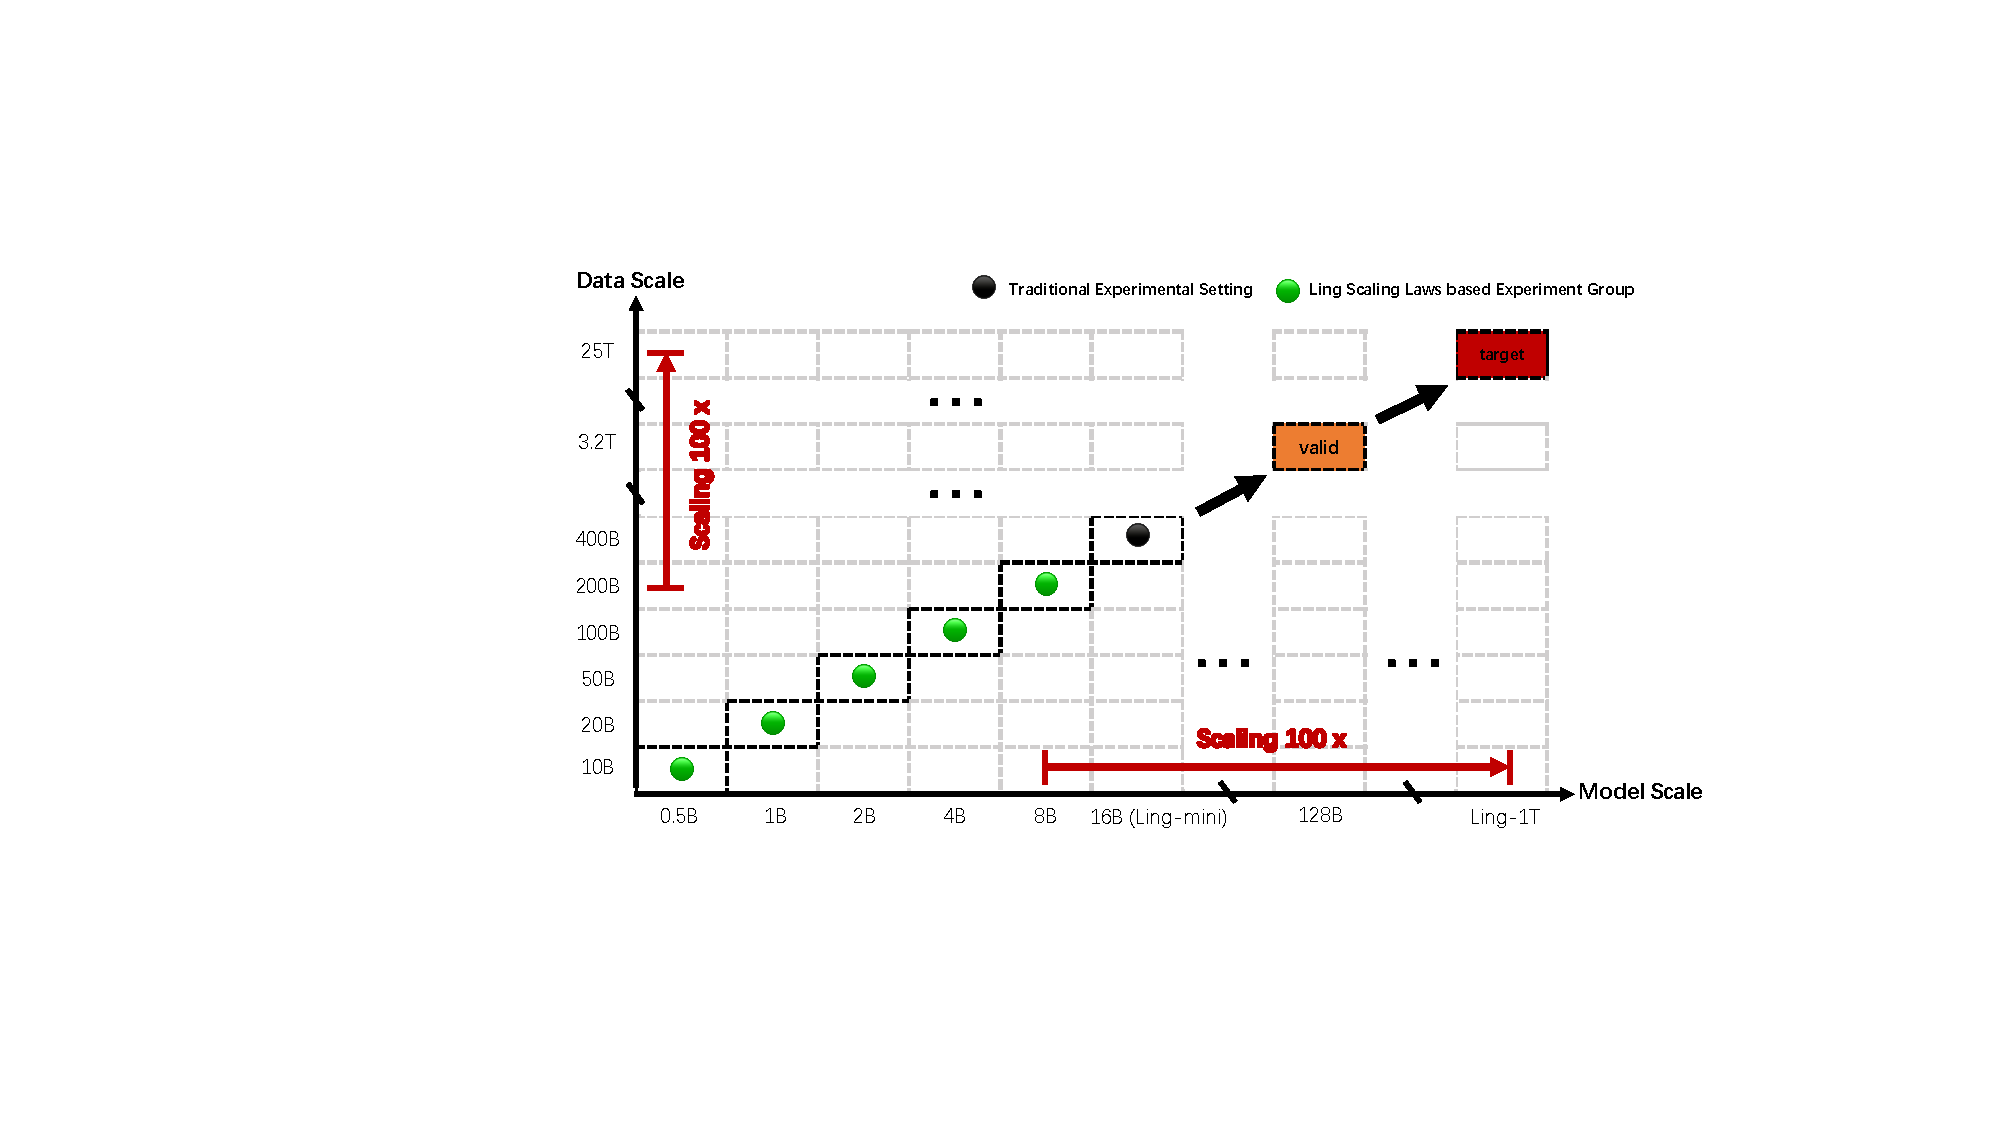
\includegraphics[width=0.9\textwidth]{figs/scaling_setting.pdf}
        \caption{Comparison Ling wind tunnel experiments and traditional experimental setting.}
        \label{fig:scaling_setting}
    \end{subfigure}
    \hfill 
    \begin{subfigure}[b]{0.42\textwidth} 
        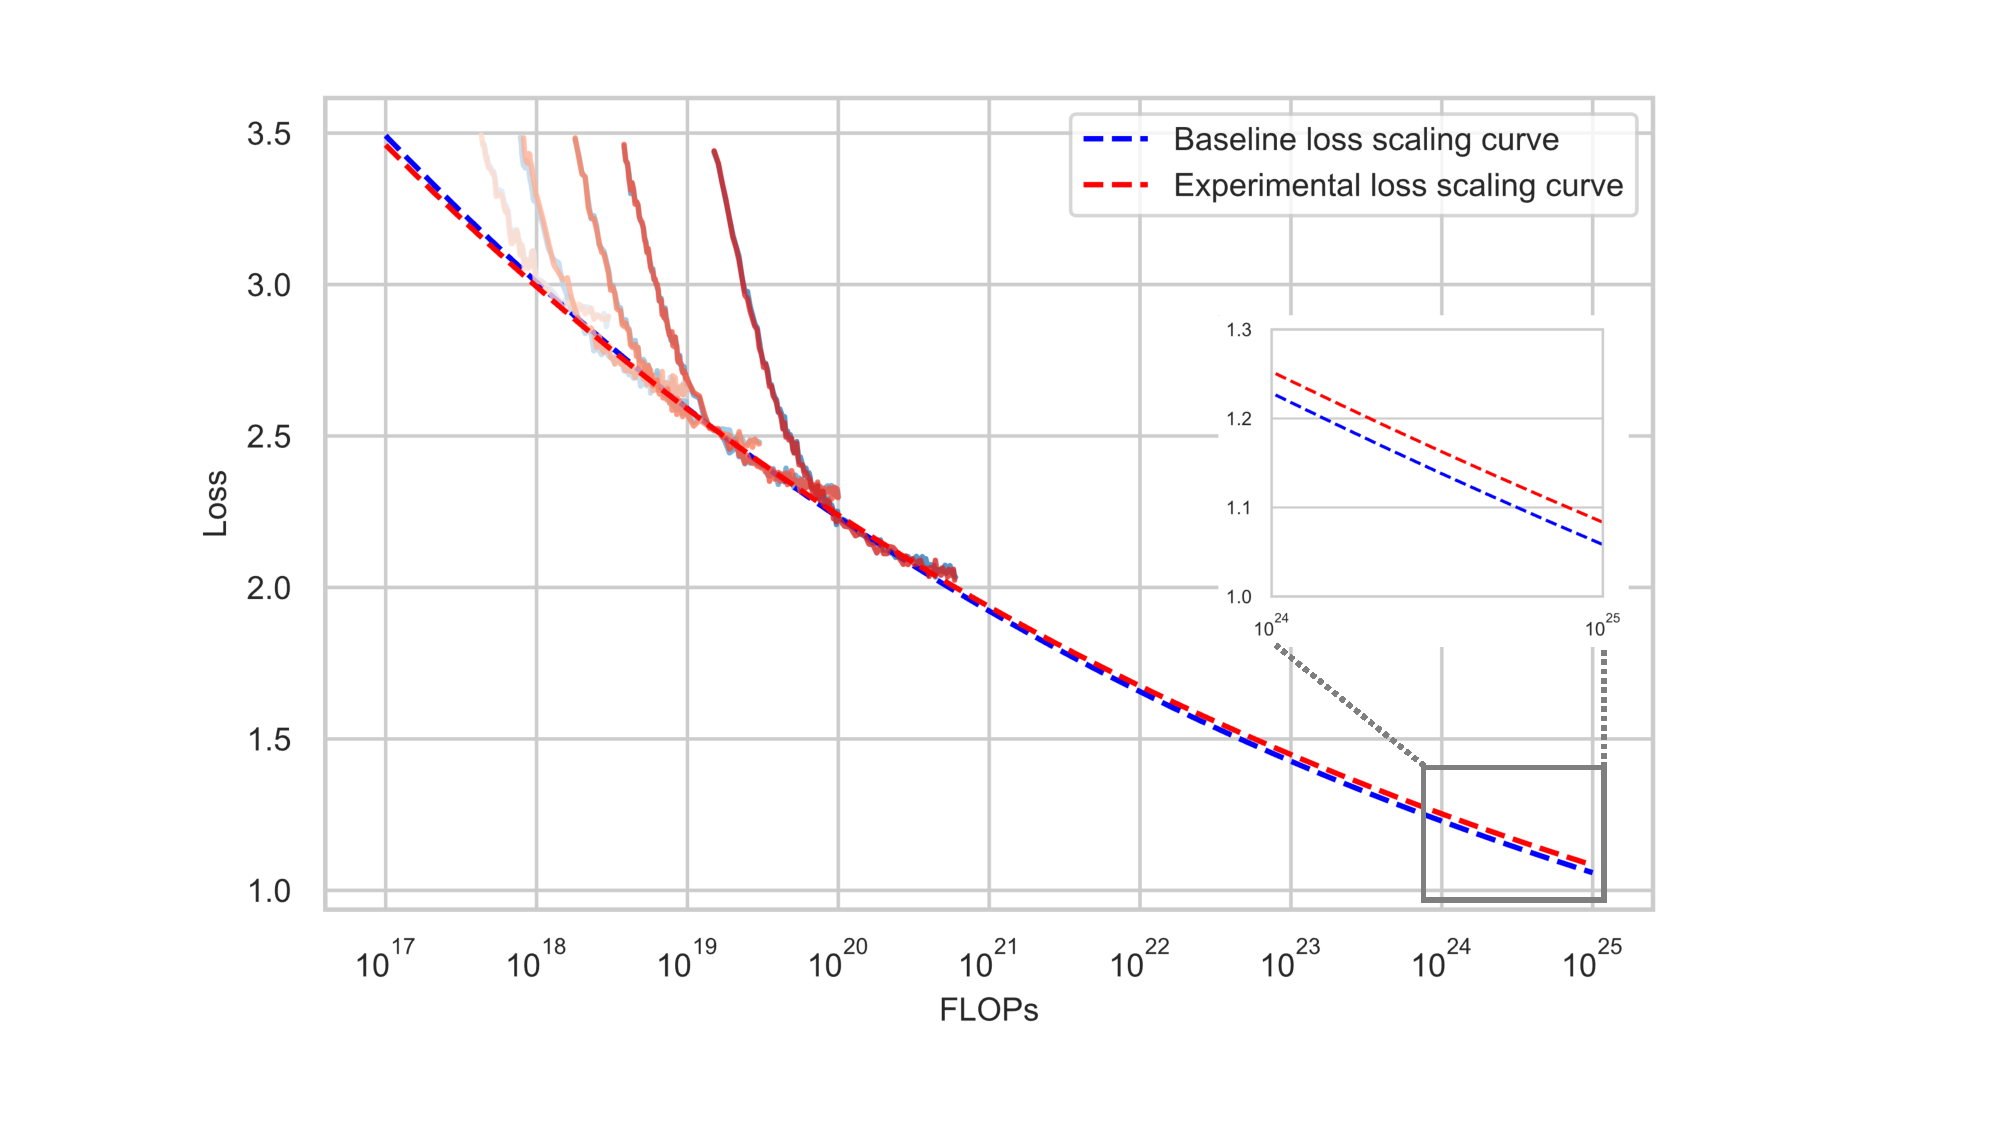
\includegraphics[width=0.9\textwidth,height=0.58\textwidth]{figs/scaling_setting_loss.pdf}
        \caption{Loss scaling curves derived by Ling wind tunnel experiments.}
        \label{fig:loss_scaling}
    \end{subfigure}
    \caption{{Illustration of the Ling Wind Tunnel's experimental design (a) and an example analysis (b).}}
    \label{fig:scaling}
\end{figure}

As depicted by the green points in Figure~\ref{fig:scaling_setting}, this system comprises five experiments with models ranging from 500M to 8B parameters, whose sizes are distributed according to a power law. The entire experimental process is highly standardized:
1) \textit{Model Architecture}: The specific architecture and size of each model are determined by the ``scaling Laws for MoE architectural efficiency'' in Secation~\ref{sec:scaling4moe}. 
2) \textit{Training Resources}: Each model is trained to a FLOPs count corresponding to its optimal compute allocation. The specific number of training tokens are determined by the ``scaling laws for optimal model-data allocation'' (Section~\ref{sec:scaling4parametres}, Figure~\ref{fig:hyper-and-modeldata-scaling-b}).
3) \textit{Training Hyperparameters}: The core training hyperparameters (i.e., learning rate and batch size) are set according to the target FLOPs, based on the ``scaling laws for optimal hyperparameters'' (Section~\ref{sec:scaling4parametres}, Figure~\ref{fig:hyper-and-modeldata-scaling-a}). 
Our experiments demonstrate that by strictly adhering to these scaling laws for hyperparameters and data allocation, we can reduce training uncertainty and accurately predict the final training loss to within an error of $0.01$. This allows the Ling Wind Tunnel system to provide automated and standardized experimental judgments, enabling us to fairly evaluate the scaling capability of any given feature. As an example shown in Figure~\ref{fig:loss_scaling}, the wind tunnel results clearly illustrate the loss difference of a candidate feature relative to the baseline across various compute budget. This provided the empirical evidence for our decisions in training the 1T foundation model. Consequently, we employ this system to identify design elements that perform well at massive scales and then extrapolate these findings 100x to guide the design of \texttt{Ling-1T}.

Compared to traditional ablation studies (e.g., training a single \texttt{\texttt{Ling-mini-2.0}} model on 400B tokens, shown as the black point in Figure~\ref{fig:scaling_setting}), the Ling Wind Tunnel is more cost-effective. Despite involving more individual runs, its overall computational cost is merely 35\% of the traditional method. More importantly, it enables us to precisely assess the scaling potential of a technology. The conclusions drawn from these multi-scale observations are significantly more stable and reliable than those derived from a single experimental ``slice.'' This methodology profoundly reflects our design philosophy for developing trillion-scale foundation models.




